\section{Étape 3 : Optimisation de la Localisation des Bureaux}
\subsection{Modélisation bi-objective}
Dans cette étape, la localisation des bureaux des représentants de vente est prise en compte comme une variable de décision supplémentaire.
L'objectif est de minimiser simultanément la distance totale parcourue et de répartir équitablement la charge de travail entre les représentants.

Soit :
\begin{itemize}
    \item $y_j$ la position du bureau du représentant $j$.
    \item $c_{jk}$ la distance entre le nouveau bureau $y_j$ et la zone $k$.
\end{itemize}

On a donc de nouveau un critère bi-objectif mais cette fois avec plus de données en entrée. 
Le premier objectif est la minimisation de la distance totale parcourue par les SR et le second objectif est la minimisation de la charge de travail maximale d'un SR. En résolvant avec Gurobi, on trouve cet espace de solutions :
\begin{figure}[H]
    \centering
    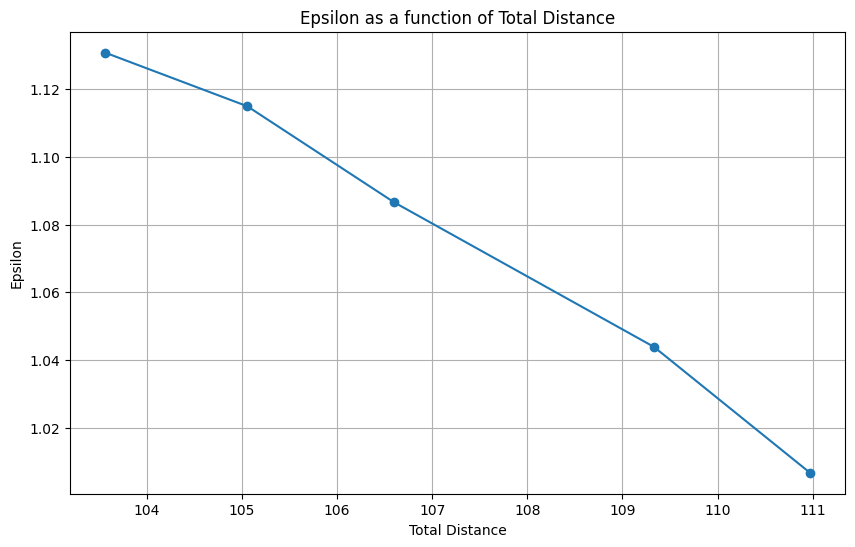
\includegraphics[width=\textwidth]{Images/step_3/bi-objective-moivng-office.png}
    \caption{Solutions non-dominées du problème bi-objectif avec la distance totale en abscisses et le MinMax de charge de travail en ordonnées}
    \label{fig:nom_de_reference}
\end{figure}


\subsection{Nouvelle disruption, nouveaux objectifs}

Maintenant, la disruption est redéfinie en termes de nombre d'office déplacé. Ainsi, le problème initial de cette étape devient tri-objectif. Comme la disruption ne peut prendre que des valeurs entières allant de 0 à 4, nous représentons les solutions non-dominées comme les graphes de solutions non-dominées bi-objectives (distance et charge de travail), à nombre d'offices changés déterminée. Voici alors l'espace des solutions :

\begin{figure}[H]
    \centering
    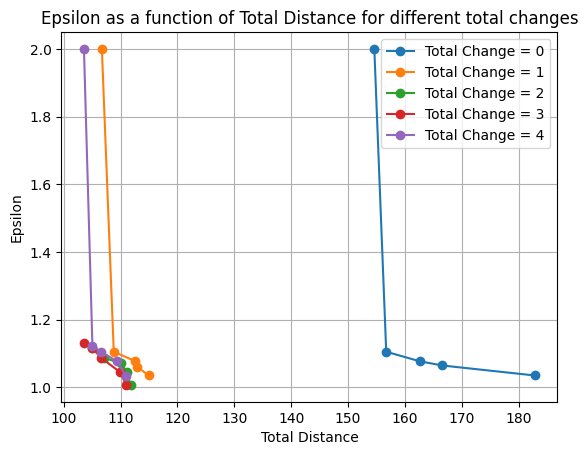
\includegraphics[width=\textwidth]{Images/step_3/tri-objectif.png}
    \caption{Solutions non-dominées du problème tri-objectif où epsilon représente le max de charge de travail pour un SR}
    \label{fig:nom_de_reference}
\end{figure}
